\documentclass[problem]{mcs}

\begin{pcomments}
  \pcomment{PS_tetris_recurrence_well_order_variant}
  \pcomment{F03.rec2 using induction}
  \pcomment{Lisa Sukharev-Chuyan revised for midterm1 2/21/17}
\end{pcomments}

\pkeywords{
  recurrence
  tetris
  tiling
}

%%%%%%%%%%%%%%%%%%%%%%%%%%%%%%%%%%%%%%%%%%%%%%%%%%%%%%%%%%%%%%%%%%%%%
% Problem starts here
%%%%%%%%%%%%%%%%%%%%%%%%%%%%%%%%%%%%%%%%%%%%%%%%%%%%%%%%%%%%%%%%%%%%%

\begin{problem}
Recall that a \emph{winning configuration} in the game of Mini-Tetris is a
complete tiling of a $2 \times n$ board using only the three shapes
shown below:

\medskip
\centerline{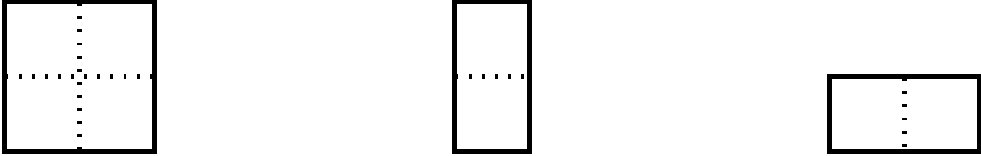
\includegraphics[height=0.5in]{rec2-tetrispieces}}

For example, here are several possible winning configurations on a $2
\times 5$ board:

\medskip
\centerline{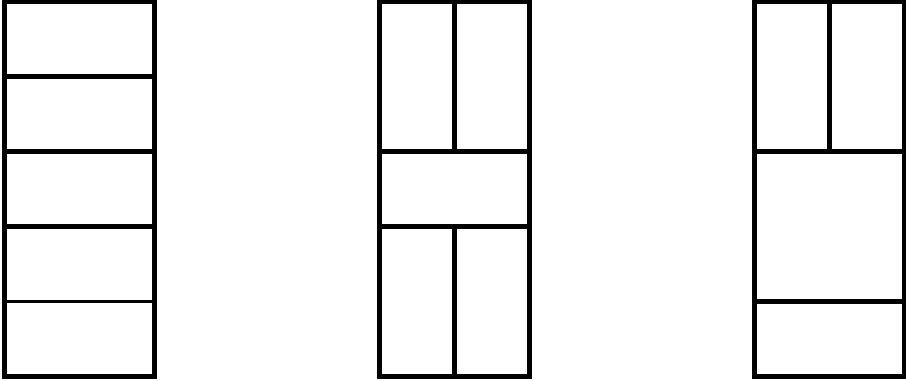
\includegraphics[height=1.25in]{rec2-2x5wins}}

\begin{problemparts}

\problempart Let $T_n$ denote the number of different winning
configurations on a $2 \times n$ board.  For example, $T_0 = 1$,
because there is exactly one way to tile a $2 \times 0$ board, that
is, use no tiles at all.

Determine the value of $T_1$.

\begin{solution}
$T_1 = 2$.
\end{solution}

\problempart\label{tnn-1n-2} Express $T_n$ in terms of $T_{n-1}$ and
$T_{n-2}$ for $n > 1$.

\begin{solution}
Every winning configuration on a $2 \times n$ board is of
one of the following three types:

\medskip
\centerline{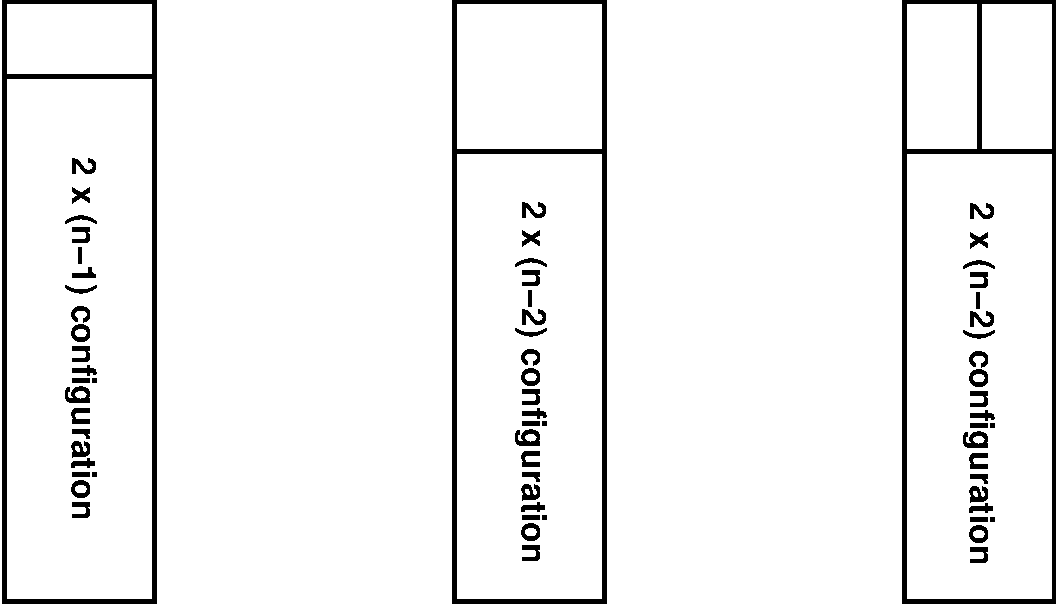
\includegraphics[height=2in]{rec2-types}}

THIS SOLUTION NEEDS TO BE UPDATED 
There are $T_{n-1}$ winning configurations of the first type, and
there are $T_{n-2}$ winning configurations of the second type and
$T_{n-2}$ again for the third type.  Overall, the number of winning
configurations on a $2 \times n$ board is:
\[
T_n  = 2 T_{n-1} + 3 T_{n-2}.
\]
\end{solution}

\problempart Use the Well Ordering Principle to prove that the number
of winning configurations on a $2 \times n$ Mini-Tetris board is:
\begin{equation}\tag{*}
T_n  = \frac{3^{n+1}+(-1)^n}{4}
\end{equation}
Hint: before you try this part, check that your answer to part b is correct.
Use your equation from part b to calculate the values of $T_2$ and $T_3$,
and check if they match the values given for $T_2$ and $T_3$ by ~(*). If not,
fix your part b!

\begin{solution}
Let $P(n)$ be the predicate
\[
P(n) \eqdef\ \brac{T_n = \frac{3^{n+1}+(-1)^n}{4}},
\]
and let $C$ be the set of counterexamples to $P$:
\[ 
C \eqdef \set{n \ge 0 \suchthat \QNOT(P(n))}.
\]

Assume for the sake of contradiction that $C$ is not empty.  Then by
the Well Ordering Principle, there is some minimum element $m \in C$.
But $P(n)$ is true for $n=0,1$:
\begin{align*}
T_0 & = 1 = \frac{3^{(0+1)}+(-1)^0}{4}, \\
T_1 & = 2 = \frac{3^{(1+1)}+(-1)^1}{4}.
\end{align*}
This means that $m$ must be greater than 1.  So both $m-1$ and $m-2$
are $\geq 0$, and since $m$ is the smallest counterexample $\geq 0$,
neither $m-1$ nor $m-2$ will be counterexamples.  Thus, we have
\begin{align*}
T_m & = 2 T_{m-1}+3T_{m-2} 
          & \text{(by part~\eqref{tnn-1n-2})}\\
    & =	2\frac{3^{m}+(-1)^{m-1}}{4} + 3\frac{3^{m-1}+(-1)^{m-2}}{4}
          & \text{(since $m-1,m-2 \notin C$)}\\
    & = \frac{2 3^{m}+(-1)^{m-1}+3^{m}+3(-1)^{m-2}}{4}\\
    & = \frac{3(2^{m})+(-2+3)(-1)^{m}}{4}\\
    & = \frac{3^{m+1}+(-1)^{m}}{4}\\
\end{align*}
This shows that $m$ satisfies~(*), so it is not a counterexample,
contradicting the definition of $m$.  So $C$ must be empty, which
proves that~(*) holds for all $n\geq 0$, as desired.
\end{solution}

\end{problemparts}

\end{problem}

\endinput
